%!TEX TS-program = ../make.zsh

\begin{frame}[fragile]{Performance}

  Time measurement: Propagating $30 \cdot 10^5$ photons on GPU.

  \begin{columns}
    \begin{column}{0.6\textwidth}
      %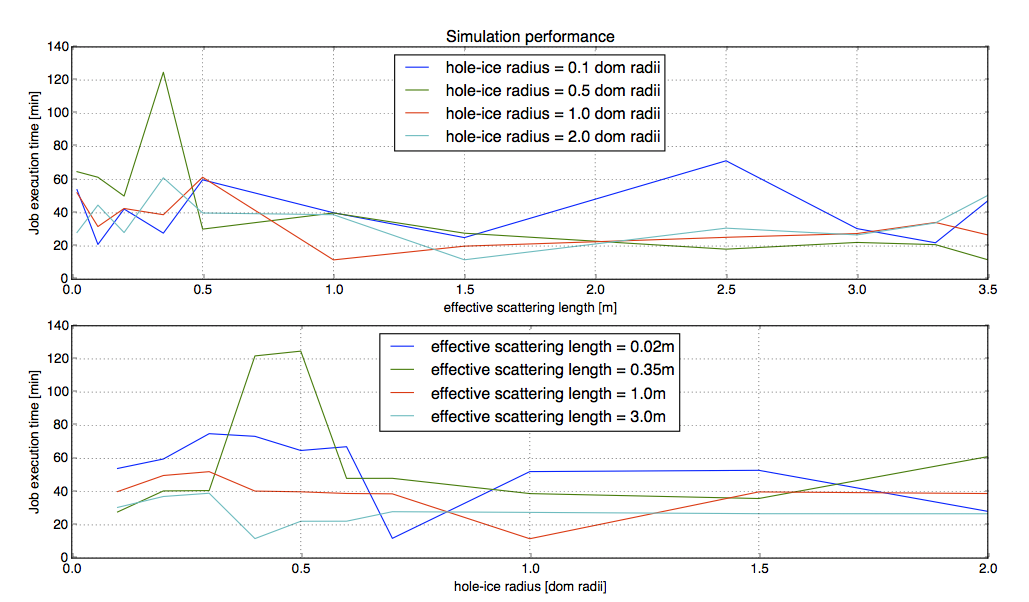
\includegraphics[width=0.8\textwidth]{img/performance-cluster-not-depending-on-hole-ice-parameters}
      \image{performance-cluster-not-depending-on-hole-ice-parameters}
    \end{column}
    \begin{column}{0.4\textwidth}
      \begin{itemize}
        \item Expectation: Simulation time increases with more demanding hole-ice properties, i.e. larger hole-ice radius and shorter scattering length.
        \item Observation: The GPU cluster node appears to determine the leading factor rather than the hole-ice parameters.
      \end{itemize}
    \end{column}
  \end{columns}

\source{https://github.com/fiedl/hole-ice-study/issues/12#issuecomment-373406819}

\end{frame}